\section{Hopf bifurcation in a cylinder wake}
\label{application_cylinder}

\subsection{The Extended Problem}

The asympotic formulation derived in the previous sections is applied to the case of the first bifurcation of a cylinder wake. The bifurcation problem has been investigated by several authors in various settings \citep{provansal87,dusek94,pier02,barkley06,giannetti07,sipp07,mantivc15,negi20}. The problem is revisited in the context of a center manifold approximation which is valid in the vicinity of the bifurcation point. 

The investigation is carried out numerically using Nek5000, an open source fluid dynamics solver originating at Argonne National Laboratory \citep{nek5000}. The code implements the spectral element method \citep{patera84}  for the Navier--Stokes equations with the $\mathds{P}_{n}-\mathds{P}_{n-2}$ formulation \citep{maday89}. The current work uses ninth order Lagrange polynomials in each direction for the representation of velocities in each spectral element and a seventh order Lagrange polynomial for the pressure with a total of $3760$ elements in the whole domain. Time integration of the system is performed using a third-order backward difference scheme with an implicit treatment of the viscous term. The non-linear terms are evaluated explicitly using extrapolation. Incompressibility is enforced using the pressure projection method \citep{deville02} implemented through the inexact LU factorization. Numerical stabilization is done using the HPF-RT method \citep{negiphd}, which adds a small amount of dissipation at the highest wavenumber scales. All quantities are non-dimensionalized using the fluid density $\rho$, the cylinder diameter $D$ and the inflow velocity $U$. The flow is characterized by the Reynolds number defined as $\Rey = UD/\nu$, where $\nu$ is the kinematic viscosity of the fluid. 

The problem domain is set up with the cylinder center located at the origin, the inflow boundary located at $x=-20$, the outflow boundary located at $x=40$ and far field boundaries located at $y=\pm20$. Dirichlet boundary condition is specified at the inflow and the standard no-stress boundary condition is applied at the outflow. The far-field boundary is equipped with the symmetry boundary condition. The bifurcation point of the system is found via a combination of selective fequency damping \citep{akervik06} for determining the fixed point of the system at each $\Rey$, along with a bisection-like algorithm for determining the point with zero growth rate. The spectral problem was solved using the Krylov-Schur algorithm \citep{stewart02}. The details of the procedure may be found in Appendix B.

The critical Reynolds number is found to be $\Rey_{c} = 46.30$ which is close to the value of $46.6$ reported in the work of \cite{sipp07}. The spectrum obtained at the bifurcation point is depicted in figure~\ref{fig:cyl_spectrum}, including the parameter mode located at the origin. The streamwise velocity for the calculated baseflow along with the parameter mode due to the extension of the system is depicted in figure~\ref{fig:base_param}. The complex conjugate pair of critical eigenvalues for the baseflow is found to be $\lambda_{c} = \pm0.7456i$, which compares well with $\lambda_{c}=\pm0.74i$ reported in \cite{sipp07}. The direct and adjoint critical eigenmodes of the flow are shown in figures~\ref{fig:flowconfig} and ~\ref{fig:flowconfig_2} respectively. The complex-conjugated mode is not shown. The modes are normalized such that the direct modes are of unit norm and the adjoint modes are scaled appropriately to maintain biorthogonality. The parameter mode is the exception where the normalization is such that $\zeta^{\dagger}_{0} = \zeta_{0} = 1$.
\begin{figure}
	\centering
	\includegraphics[width=0.49\textwidth]{baseflow0000}
	\includegraphics[width=0.49\textwidth]{dirmode0000}
	\caption{Streamwise velocity of (top) the stationary base flow at $\Rey_{c}=46.30$ and (bottom) the parameter mode.}
	\label{fig:base_param}
\end{figure}	

\begin{figure}
	\centering
	\includegraphics[width=0.49\textwidth]{cyl_spectra}
	\caption{Spectrum for the flow across a cylinder at the critical Reynolds number of $Re_{c}=46.30$. The spectrum includes the parameter mode located at the origin.}
	\label{fig:cyl_spectrum}
\end{figure}	

%\begin{figure}
%	\includegraphics[width=0.49\textwidth]{dirmode0001}
%	\includegraphics[width=0.49\textwidth]{dirmode0002}
%	\includegraphics[width=0.49\textwidth]{adjmode0001}
%	\includegraphics[width=0.49\textwidth]{adjmode0002}
%	\caption{Streamwise velocity of the eigenmodes. From top to bottom the figures represent the: real part of the direct critical mode, imaginary part of the direct critical mode, real part of the adjoint critical mode and, imaginary part of the adjoint critical mode.}
%	\label{fig:flowconfig}
%\end{figure}

\begin{figure}
	\includegraphics[width=0.49\textwidth]{dirmode0001}
	\includegraphics[width=0.49\textwidth]{dirmode0002}
	\caption{Streamwise velocity of the direct eigenmode. The panels represent the (top) real part and (bottom) imaginary part of the direct critical mode.}
	\label{fig:flowconfig}
\end{figure}

\begin{figure}
	\includegraphics[width=0.49\textwidth]{adjmode0001}
	\includegraphics[width=0.49\textwidth]{adjmode0002}
	\caption{Streamwise velocity of the adjoint eigenmode. The panels represent the (top) real part and (bottom) imaginary part of the adjoint critical mode.}
	\label{fig:flowconfig_2}
\end{figure}


\subsection{Asymptotic Center Manifold Approximation}

For a second order asymptotic approximation of the graph $\mathfrak{h}(\mathbf{x})$, one obtains six fields $\vpfield{y}_{i,j}$, that are solutions to the restricted resolvent equations~\eqref{second_order_expressions}, corresponding to the fields associated with the terms $x_{i}x_{j}$ in the series expansion of $\mathfrak{h}$, where, $i,j\in 0,1,2;\ j \ge i $. The fields are in general complex with the exception of $\vpfield{y}_{0,0}$ and $\vpfield{y}_{1,2}$, which are restricted resolvent solutions at zero frequency and are purely real fields. The fields $\vpfield{y}_{0,0}$ and $\vpfield{y}_{1,2}$ are depicted in figure~\ref{fig:resolvents_zero}. These, in combination with the parameter mode, provide contributions to what is often termed as the mean flow correction.
\begin{figure}
	\centering
	\includegraphics[width=0.49\textwidth]{real_resmode0000}
	\includegraphics[width=0.49\textwidth]{real_resmode0004}							
	\caption{Streamwise velocity components of the restricted resolvent solutions corresponding to the zero frequency fields (top) $\vpfield{y}_{0,0}$ and (bottom) $\vpfield{y}_{1,2}$.}
	\label{fig:resolvents_zero}
\end{figure}

The real and imaginary parts of the resolvent solution fields $\vpfield{y}_{0,1}$ and $\vpfield{y}_{1,1}$ are depicted in figure~\ref{fig:resolvents_oscillatory_real} and ~\ref{fig:resolvents_oscillatory_imag}. The fields $\vpfield{y}_{0,1}$ and $\vpfield{y}_{0,2}$ are complex-conjugate pairs, and likewise for $\vpfield{y}_{1,1}$ and $\vpfield{y}_{2,2}$ (the complex conjugated fields are not displayed). These are the oscillatory solutions of the second order asymptotic approximation of $\mathfrak{h}$. The angular frequencies of $\vpfield{y}_{0,1}, \vpfield{y}_{0,2}, \vpfield{y}_{1,1}, \vpfield{y}_{2,2}$ are the imaginary parts of $\lambda_{c},-\lambda_{c},2\lambda_{c}$ and $-2\lambda_{c}$ respectively. 
%\begin{figure}
%	\centering
%	\begin{subfigure}[t]{0.49\textwidth}
%		\includegraphics[width=1.00\textwidth]{real_resmode0001}
%		\includegraphics[width=1.00\textwidth]{imag_resmode0001}
%		\label{fig:x0x1_r_i}
%	\end{subfigure}
%	\begin{subfigure}[t]{0.49\textwidth}
%		\includegraphics[width=1.00\textwidth]{real_resmode0003}
%		\includegraphics[width=1.00\textwidth]{imag_resmode0003}
%		\label{fig:x1x1_r_i}
%	\end{subfigure}		
%	\caption{The panels depict the streamwise velocity components of the solution fields $\vpfield{y}_{i,j}$. From top to bottom the fields represent the: real part of $\vpfield{y}_{0,1}$, imaginary part of $\vpfield{y}_{0,1}$, real part of $\vpfield{y}_{1,1}$ and imaginary part of $\vpfield{y}_{1,1}$, with angular frequencies equal to the imaginary parts of $\lambda_{c}$ and $2\lambda_{c}$.}
%	\label{fig:resolvents_oscillatory}
%\end{figure}
\begin{figure}
	\centering
	\includegraphics[width=0.49\textwidth]{real_resmode0001}
	\includegraphics[width=0.49\textwidth]{real_resmode0003}
	\caption{The panels depict the real part of the streamwise velocity components of (top) $\vpfield{y}_{0,1}$ and (bottom) $\vpfield{y}_{1,1}$ with angular frequencies equal to the imaginary parts of $\lambda_{c}$ and $2\lambda_{c}$.}
	\label{fig:resolvents_oscillatory_real}
\end{figure}
\begin{figure}
	\centering
	\includegraphics[width=0.49\textwidth]{imag_resmode0001}
	\includegraphics[width=0.49\textwidth]{imag_resmode0003}
	\caption{The panels depict the imaginary part of the streamwise velocity components of (top) $\vpfield{y}_{0,1}$ and (bottom) $\vpfield{y}_{1,1}$ with angular frequencies equal to the imaginary parts of $\lambda_{c}$ and $2\lambda_{c}$.}
	\label{fig:resolvents_oscillatory_imag}
\end{figure}
Once the fields $\vpfield{y}_{i,j}$ have been evaluated, substitution in to equation~\eqref{amplitude_second_oder} then results in the coefficients of the polynomial terms $x_{i}x_{j}$ and $x_{i}x_{j}x_{k}, \ (i,j,k \in 0,1,2;\ j\ge i; k\ge j)$ of the center-manifold amplitude equations. When the graph equation is evaluated asymptotically at second order the resulting center-manifold equations are of third order (in $\mathbf{x}$). Since $x_{1}$ and $x_{2}$ are the amplitudes of the complex-conjugated pair of modes, the resulting expressions for the center-manifold amplitude equations obtained for the two variables are also complex-conjuated with respect to the other. Differences arise due to the numerical accuracy of the terms evaluated and in the current work this complex-conjugacy property is violated at $\mathcal{O}(10^{-8})$. A full list of the evaluated terms is given in the appendix. The combinatorial problem would allow a total of $19$ terms for each equation however, a significant number of the terms are of the order of the convergence tolerance used for the spectral solver and are treated as negligible. Even the inhomogeneous terms $x_{0}x_{0}$ and $x_{0}x_{0}x_{0}$ are negligible in the current case under examination. The vanishing of several terms in the center-manifold amplitude equations may also be deduced by inspecting the spatial symmetry of the resulting terms. Replacing $x_{1},x_{2}$ with $x,x^{*}$, and $x_{0}$ with the parameter variable $\eta$, and ignoring the small terms ($<10^{-5}$), one obtains the following equation for $\dt{x}$
\begin{equation}
	\label{numerical_amplitude_eqn_x1_p1}
	\begin{aligned}
			\dt{x} =& +[0.7456i]x \\
			%
			& + [(1.976 + 0.698i)\times10^{-1}]\eta x \\ 
			%
			& + [(6.388 + 4.616i)\times10^{-3}]\eta x^{*}  \\
			%
			& + [(7.264 - 4.787i)\times10^{-2}]\eta^{2} x \\
			%
			& + [(4.477 - 1.482i)\times10^{-3}]\eta^{2}x^{*} \\
			%
			& + [(1.615 - 2.904i)\times10^{-5}]x^{3}  \\
			%
			& - [(2.526 - 8.010i)\times10^{-3}](x^{*}x)x \\
			%
			& + [(0.973 - 3.380i)\times10^{-5}](x^{*}x)x^{*} \\
			%
		\end{aligned}
\end{equation}
The complex conjugation of equation~\eqref{numerical_amplitude_eqn_x1_p1} results in the equation for $\dt{x}^{*}$. The equation may now be evaluated numerically to obtain the time history and the resulting non-linear angular frequency of the reduced system. The evolution of the system at a parameter value of $\eta=0.074$ ($\Rey=50.0$) is shown in figure~\ref{fig:center_manifold_evolution}, depicting the typical evolution to the saturated limit cycle. 
\begin{figure}
	\centering
	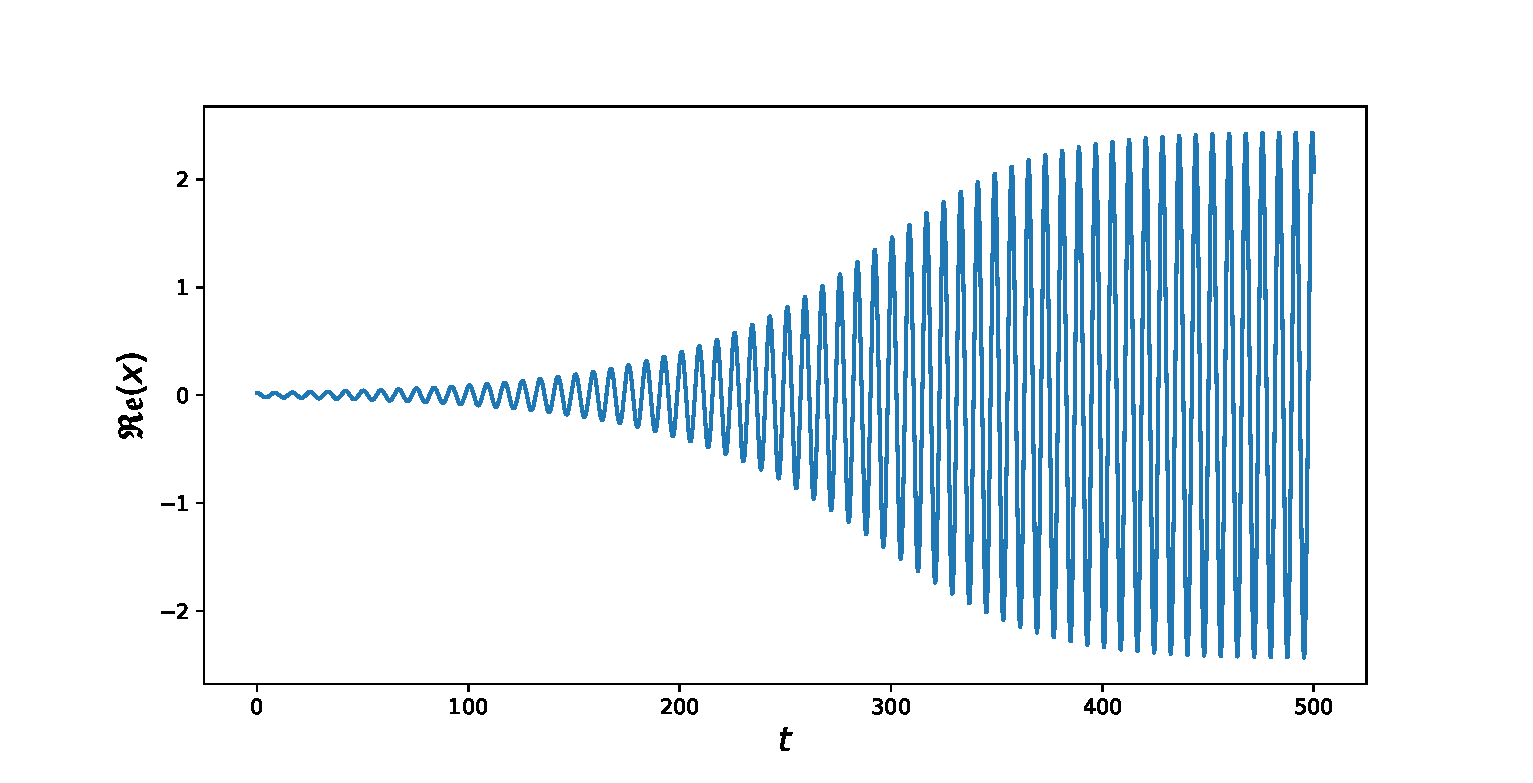
\includegraphics[width=0.50\textwidth]{center_manifold_evolution}	
	\caption{The time evolution of the real part of $x$ via the center-manifold amplitude equations. The system is evaluated at $\eta=0.074$}
	\label{fig:center_manifold_evolution}
\end{figure}
The center-manifold amplitude equations are numerically integrated for several different parameter values and the angular frequency of the limit cycle oscillations is obtained. The comparison between the frequencies obtained through the full non-linear simulations and those obtained through the reduced center-manifold amplitude equations is show in figure~\ref{fig:limit_cycle_frequency}. Close to the bifurcation point the saturated limit-cycle frequencies are well predicted by the reduced equations however, as the Reynolds number increases the saturation frequency systematically deviates from the results of the full non-linear simulations. Recall that the the center-manifold reduction is only an asymptotic approximation, therefore higher order terms could provide contributions as the system is moved away from the critical point. Alternately, the center-manifold approximation itself may not be valid sufficiently far away from the critical point, so that the solution $\vpfield{u}_{s}$ which lies in the stable subspace can no longer be assumed to evolve as a graph of the critical subspace. 
\begin{figure}
	\centering
	\begin{subfigure}[t]{0.49\textwidth}
		\includegraphics[width=1.0\textwidth]{center_manifold_omega}
		\caption{}
		\label{fig:limit_cycle_frequency}
	\end{subfigure}	
	\begin{subfigure}[t]{0.49\textwidth}
		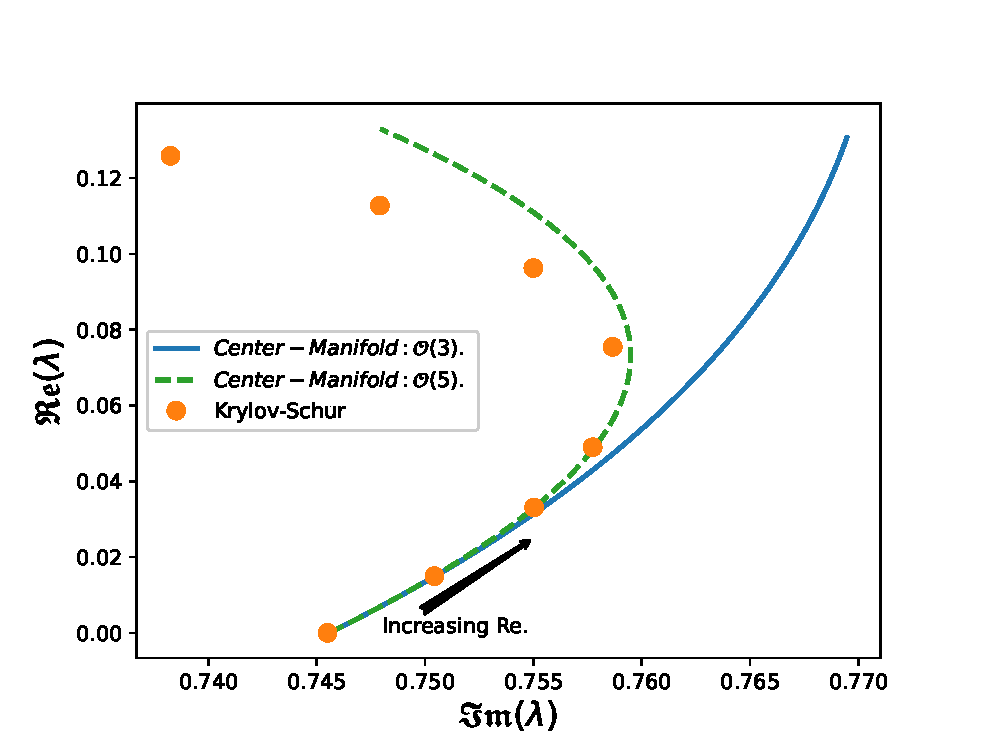
\includegraphics[width=1.0\textwidth]{spectra_comparison}
		\caption{}
		\label{fig:linearized_eigenvalue}
	\end{subfigure}									
	\caption{Comparison of the linear and non-linear angular frequencies of the full system and the center-manifold amplitude equations. (a) Comparison of the angular frequencies of the saturated limit cycles at different Reynolds numbers. (b) Comparison of the linearized system eigenvalue (with positive imaginary part) for varying Reynolds numbers.}
	\label{fig:frequency_comparison}
\end{figure}

In addition to the saturated limit cycle angular frequency one may also estimate the variation of the linearized angular frequency \ie the eigenvalue of system beyond the critical point through the reduced equations. Since the inhomogeneous terms in the reduced system are negligible, the variation of the eigenvalue as a function of the parameter $\eta$ is directly obtained from the linear terms  in equation~\eqref{numerical_amplitude_eqn_x1_p1}. A comparison of the obtained eigenfrequencies of the center-manifold equations ($\mathcal{O}(\mathbf{x}^{3})$) and those computed for the full system using the Krylov-Schur algorithm for different Reynolds numbers is shown in figure~\ref{fig:linearized_eigenvalue}. Close to the critical point the variation of the eigenvalue seems to be fairly well captured by the reduced equations. In an attempt to obtain a better asymptotic approximation higher order terms up to $\mathcal{O}(\mathbf{x}^{4})$ were evaluated resulting in a fifth order equation for the center-manifold amplitudes. However, at this order the highest order term $(|x|^{4}x)$ has a coefficient with a positive real part, leading to an unbounded system. Presumably one needs to evaluate $\mathfrak{h}(\mathbf{x})$ to $\mathcal{O}(\mathbf{x}^6)$ to obtain a bounded reduced system again (in which case the center-manifold amplitude equations would be of $\mathcal{O}(\mathbf{x}^{7})$). Further higher order approximations have not been pursued. One may nonetheless obtain a higher-order estimate of the linearized frequencies of the reduced system from this higher order (but unbounded) system ($\mathcal{O}(\mathbf{x}^{5})$). This is plotted in figure~\ref{fig:linearized_eigenvalue} with a dashed line. Clearly the higher order estimate follows the eigenvalues of the full system much more closely, providing evidence for the conjecture that the higher order terms of the asymptotic approximation do indeed have significant contribution as the system moves away from the critical point.

\subsection{The Stuart-Landau equation}
\label{stuart_landau}

The Landau model has often been utilized to understand the behavior of weakly unstable systems close to the bifurcation point \citep{dusek94,sipp07,carini15,meliga12}. The original model was proposed by Landau based on symmetry, scaling and phenomenological arguments \citep{landau_52}. In the hydrodynamics literature the model is referred to as the Stuart-Landau equation and was first obtained through energy considerations in \cite{stuart58} and via the separation of time scales in \cite{stuart60,watson60}. In order to transform the center-manifold amplitude equations to a form similar to the Stuart-Landau equation, one may multiply equation~\eqref{numerical_amplitude_eqn_x1_p1} with $x^{*}$, and multiply the the complex-conjugate of equation~\eqref{numerical_amplitude_eqn_x1_p1} with $x$. Adding the two resulting equations together leads to an equation for the squared amplitude $x^{*}x = |x|^{2}$. One may then follow the phenomenological arguments of \cite{landau_52} for the evolution of the amplitudes in the case of small linear growth rates. Assuming that the system is close to the bifurcation point and the instability is weak, then the change in the amplitude over one cycle of the fundamental frequency also remains small. In such a scenario the evolution equation for the squared amplitude may be averaged over one cycle to obtain the evolution of the average amplitude. The averaging process causes all the oscillatory terms of the type $(x)^{2},(x^{*})^{2},|x|^{2}(x),|x|^{2}(x^{*})$ \textit{etc.} to (nearly) vanish, and the only remaining terms are those related to the modulus of the amplitude. Representing the averaged modulus as $|A|^{2} = \overline{|x|^{2}}$, one obtains the Landau model for the problem as
\begin{equation}
	\label{landau_eqn_1}
		\dfrac{d|A|^{2}}{dt} = 2\times[0.1976\eta + 0.0726\eta^{2}] |A|^{2} - 0.0051|A|^{4}.
\end{equation}
The arguments presented by Landau correspond to the more formal procedure of multiple time-scale expansion and the averaged amplitude $|A|$ corresponds to the amplitude modulation governed by the slow time-scale equations (usually obtained through the solvability condition).

While this is not undertaken in the original work of \cite{landau_52}, a similar procedure may be invoked to obtain a slow drift of the angular frequency. Representing $x = |A|e^{i\theta} = |A|e^{i\phi(t)}e^{\lambda_{c}t}$, where, $\phi(t)$ represents the slowly varying drift in angular frequency and $\lambda_{c}$ the critical eigenvalue of the system. One may substitute this expression into equation~\eqref{numerical_amplitude_eqn_x1_p1} and subtract the complex conjugated equation (corresponding to the equation for $x^{*}$) to obtain an expression for $\dt{\phi}$. This equation again contains oscillatory terms of the type $e^{\lambda_{c}t},e^{-\lambda_{c}t},e^{2\lambda_{c}t},e^{-2\lambda_{c}t}$ \textit{etc}. These may be eliminated by averaging over the fundamental time period of the oscillation, with the assumption that $\phi(t)$ remains nearly constant during one cycle of the oscillation, resulting in the expression,
\begin{equation}
	\label{landau_eqn_2}
	\dfrac{d\phi}{dt} = [0.0698\eta - 0.0478\eta^{2}]  + 0.0080|A|^{2}.
\end{equation}
Combining the two equations in $A = |A|e^{i\phi(t)}$ and using the definition of the derivatives in equations~\eqref{landau_eqn_1} and \eqref{landau_eqn_2} one obtains
\begin{eqnarray}
	\label{stuart_landau_eqn}
	\begin{split}
		\dt{A} 					=& [(0.1976 + i0.0698)\eta + (0.0726 - i0.0478)\eta^{2}] A \\
										& - \frac{1}{2}[0.0051 - i0.0160]|A|^{2}A.
	\end{split}
\end{eqnarray}
This is the amplitude equation or, the Stuart-Landau equation for the case in question. In its normal form the Stuart-Landau equation is represented as $\dt{A} = (\sigma_{r} + i\sigma_{i})A - 1/2(l_{r} + il_{i})|A|^{2}A$, and the correspondence is seen immediately. Equation~\eqref{stuart_landau_eqn} may be derived more formally through the usual procedure of multiple time-scale expansion. This however is not undertaken and the phenomenological arguments are deemed sufficient, especially given that a reduced system of center-manifold amplitude evolution has already been obtained in equation~\eqref{numerical_amplitude_eqn_x1_p1}. The Landau constant is found to be $l_{r} = 0.0051$, however, this constant depends on the normalization of the global mode. The ratio $l_{i}/l_{r} = -3.14$ is independent of the normalization. There appears to be some amount of scatter in the reported values of this ratio in the literature, with reported value being $-2.7$  in \cite{dusek94}, $-3.42$ in \cite{sipp07}, $-3.3$ in \cite{meliga12}, and $-3.63$ in \cite{carini15}. The value found in the current work seems to be within the scatter reported in the literature and the reasons behind the scatter are not entirely clear. The ``growth-rate'' of the amplitude that varies linearly with $\eta$ is found here to be $\sigma_{r}=0.1976$ which at first glance appears to be very different from the values reported in \cite{sipp07,meliga12,carini15}. However, in the current work $\eta$ is scaled with $\invRec$  and upon rescaling its value is $9.1488$, which matches well with the values reported in the literature.



